%%report template for pattern recognition SS2016

\documentclass[english, paper=a4]{scrartcl}
\usepackage[utf8]{inputenc}
% images
\usepackage{graphicx}
%math
\usepackage{amsmath,amssymb}
%code
\usepackage{algorithm}
\usepackage[noend]{algpseudocode}
\makeatletter
\def\BState{\State\hskip-\ALG@thistlm}
\makeatother

\usepackage{subcaption}
\captionsetup{compatibility=false}
\usepackage{multirow}
\usepackage{color}
\usepackage{enumitem}


\begin{document}

\graphicspath{{images/}}


%%------------------------------------------------------
%% provide your input here:
\title{Assignment 1 - Page Detection} 

\subtitle{Document Analysis} 

\author{Timon Höbert(01427936) \\ Manuel Mayerhofer (01328948)\\ Stefan Stappen(01329020)}



%%------------------------------------------------------

\maketitle


%%------------------------------------------------------

\section{Definition of Task}
Optical character recognition is the task of transforming digitalized documents again into a machine readable format.
Precisely, the content of images of documents is analysed, characters are recognized and the text is rebuilt from the characters. The ICDAR2015Competition on Smartphone Document Capture and OCR (SmartDoc) \cite{burie2015icdar2015} is the first competition for document page detection and Smartphone OCR. The second assignment of this competition was OCR.\\
The input is a scanned in document, a subset of the "I AM printed" dataset. The output represents the text inside the document with x and y coordinates for each character.

\section{Dataset}
The dataset consists of a subset of the I AM PRINTED dataset. The images are all 2 to 7 lines of text with negligible
skew. For this reason we omitted the skew detection. Every text has a enclosing lines at the top and the bottom
and sometimes there is handwritten text at the bottom. All the text samples are written with the same style, with serifs,
none-bold and the same font-art. There are only minor changes in resolution.
The whole dataset consists of 100 images and 100 xml files containing the ground truth. In each xml file
x and y coordinates for each line, word and character can be found. Though, these seem not be correct as width and height
exceed the resolution of the images!

\section{Implementation}
As recommended, we implemented for the line, word and character segmentation projection profiles. 
Our OCR is based on a trained neural network. For this reason, we created our own training data and annotated them
semi-automatically. TODO
For the neural networks we used the python library TODO


\subsection{Line, Word and Character Segmentation}
In a preprocessing step, we eliminate noise with a Gaussian blur. Afterwards, we threshold the image with 
an Otus-Threshold and invert the image. In the next step we dilate the image for better line segmentation.

After the preprocessing we are ready to compute the horizontal projection profile. In figure \ref{fig:ex_proj_horz}
a preprocessed image and its horizontal projection profile can be observed.

Word segmentation

Character Segmentation
no Gaussian blur, even tried Skeletonization  

\begin{figure}[b!]
	\centering
	\begin{subfigure}[t!]{0.30\textwidth}
		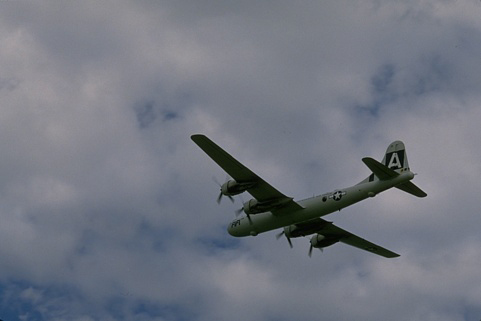
\includegraphics[width=\textwidth]{3096.jpg}
		\caption{preprocessed image}
		\label{fig:ex2a}
	\end{subfigure}
	\begin{subfigure}[t!]{0.30\textwidth}
		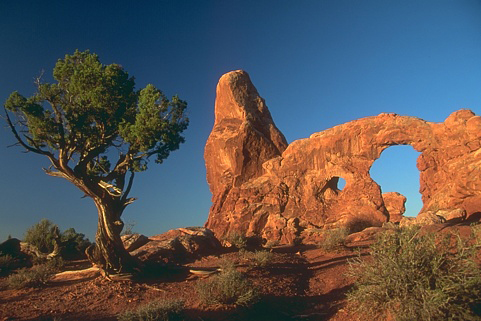
\includegraphics[width=\textwidth]{295087.jpg}
		\caption{horizontal projection profile}
		\label{fig:ex2b}
	\end{subfigure}
	\caption{Example images from Berkeley segmentation database \cite{martin01}.}
	\label{fig:ex_proj_horz}
\end{figure}

\section{Performance}
TODO
One big drawback of the algorithm is the execution time that depends on the number of founded line segments. We calculate for every combination of two horizontal and two vertical lines a bounding box. This is very expense even with a small number of lines due to the permutations. Another problem is that the LSD algorithm takes only an input image path as input. So we have to create an image for every frame and write it out.

\section{Evaluation}
TODO
To measure the performance the Jacard index measure \cite{everingham2010pascal} is used. 
The Jacard index is the intersection of the detected bounding box with the ground truth document bounding box divided through the union of the bounding boxes (see equation \ref{eq:1}).
\begin{equation}\label{eq:1}
JI(frame)= \frac{area(G\cap S))}{area(G\cup S))}
\end{equation}

The score for one video is the average of the frame scores, and the overall accuracy of the implemented method is the average of all videos with different backgrounds.

\section{Results}

The computed Jacard indices for the given dataset with our method can be viewed in 
table \ref{tab:results}.

\begin{table*}[]
\centering
\caption{Jacard Index Results}
\label{tax}
\begin{tabular}{l | p{2cm}| p{2cm}| p{2cm}| p{2cm}| p{2cm} }
\hline
& \multicolumn{5}{|c}{\textbf{Background}} \\
\textbf{Document Type} &  \multicolumn{1}{c}{01} & \multicolumn{1}{c}{02} & \multicolumn{1}{c}{03} & \multicolumn{1}{c}{04} &\multicolumn{1}{c}{05} \\ \hline\hline
Datasheet & 0.961804   & 0.933321  &0.956437 &0.338121 &0.419252  \\ 
           &0.969550 & 0.949776  &0.953702 &0.670783 &0.204255  \\ 
           & 0.958112  & 0.926158  &0.954332 &0.460790 &0.407288  \\ 
           & 0.963166  & 0.942556  &0.957530 &0.406976 &0.279959  \\ 
           & 0.956819  & 0.931061  &0.964136 &0.480986 &0.373999  \\ \hline
Letter & 0.966585 & 0.931361  &0.964660 &0.548722 &0.488031  \\    
		& 0.962465 & 0.950924  &0.939243 &0.637083 &0.454185  \\ 
		& 0.962962 & 0.943569  &0.901809 &0.444535 &0.463177  \\ 
		& 0.955535 & 0.945724  &0.939415 &0.690977 &0.405386  \\ 
		& 0.959804 & 0.939154  &0.941210 &0.414960 &0.624913  \\ \hline 
Magazine & 0.961872 & 0.906609  &0.945897 &0.169548 &0.042877  \\   
		& 0.959672 & 0.937086  &0.919084 &0.148990 &0.110548  \\ 
		& 0.922668 & 0.900296  &0.941420 &0.693086 &0.000000  \\ 
		& 0.886081 & 0.863409  &0.915656 &0.389279 &0.552460  \\ 
		& 0.922554 & 0.813186  &0.964260 &0.458704 &0.175053  \\ \hline 	
Paper & 0.956659 & 0.967295  &0.952133 &0.667463 &0.410692  \\   
		& 0.954750 & 0.959377  &0.904080 &0.610046 &0.015565  \\ 
		& 0.943191 & 0.955013  &0.950578 &0.557951 &0.408258  \\ 
		& 0.923238 & 0.947480  &0.971184 &0.643748 &0.447700  \\ 
		& 0.954222 & 0.934069  &0.962020 &0.614676 &0.453615  \\ \hline 	
Patent & 0.944150 & 0.950614  &0.915164 &0.629440 &0.464737  \\   
		& 0.934623 & 0.942731  &0.906549 &0.634424 &0.380177  \\ 
		& 0.939969 & 0.935944  &0.956033 &0.538994 &0.502359  \\ 
		& 0.944970 & 0.918508  &0.897266 &0.226930 &0.358804  \\ 
		& 0.914572 & 0.837318  &0.954834 &0.548980 &0.311188  \\ \hline 
Tax & 0.949686 & 0.902505  &0.944010 &0.342882 &0.490883  \\   
		& 0.940098 & 0.937493  &0.956152 &0.575945 &0.016099  \\ 
		& 0.867588 & 0.938492  &0.933569 &0.466925 &0.062252  \\ 
		& 0.903321 & 0.880571  &0.936461 &0.419935 &0.047539  \\ 
		& 0.951203 & 0.932429  &0.930931 &0.249198 &0.500233  \\ 	\hline \hline 
\textbf{Overall/Background} &0.9431 & 0.9251 & 0.9410 & 0.4894 &0.3290\\ \hline 
\textbf{Overall}&	 0.7255					            
\end{tabular}
\label{tab:results}
\end{table*}

We tried to optimize our approach for the usual case of page detection
with a smartphone. For this reason we optimized our technique for the first three
datasets. 
The fourth background is not really in a natural environment because usually 
the flash light is turned of during video page detection with a smartphone,
though this case is arguable. 
The fifth background does not make any sense as the later for OCR needed
information is anyway overlayed by other stuff. Although, there are more
than one document and it can be argued to decide which document to detect.

Anyway, we tried to improve our solution even for these unrealistic cases.
First we had to tackle that because of missing contrast and overlays not the 
right lines were detected by the LSD.
To overcome this proble, we convert the image in a gray value image. Then we use the canny edge detector with a sigma of 3 to create a binary image of the document. We chose the canny detector because it found most of the edges in the document frames, unlike Sobel or Prewitt. However, there were many distortions on the edges, so we increased the sigma from $\sqrt{2}$ to 4 to smooth the image a bit. The result of the preprocessing steps looks like Figure \ref{fig:pre}.

With this preprocessing step the LSD again finds reasonable lines for the datasets
with background four and five. Though, the results only improved to about 60 \%.
For the realistic backgrounds, one, two and three this preprocessing step has a severe impact. Due to the loss of information by converting the image into an edge image,
the important lines get lost for the realistic data sets.
The results are reduced from over 90 \% to about 60 \%. 
For this reason we stayed without the preprocessing step and 
therefore created a method which works quite well for realistic scenarios
(over 90 \%) and fails at unrealistic scenarios, a justifiable trade-off.

It is still to be noted, that for none of the described methods using LSD
a paper could be found. Maybe they changed the method name or someone else
in their research group published the paper with another name
because we searched for the method names and the authors and could not find the papers.
If they really did not publish there methods it is arguable that 
the description is either not complete and some other
criteria for bounding box selection is used or that they optimized
the parameters for the given datasets to achieve these results.

\newpage
\bibliographystyle{plain}
\bibliography{lit}
%% References can be stored in a seperate bib-file (see lit.bib). References, that are cited in the report using \cite are automatically added to the reference list. For more information: http://www.bibtex.org/Using/
%%------------------------------------------------------
\end{document}
